% TeX шаблон, пример оформления отчёта по лабораторной работе.
% Автор: Шмаков И.А.
% Версия от: 05 ноября 2018 года.
% Сборка документа из командной строки:
% ~$ pdflatex -shell-escape main.tex

\documentclass[a4paper,14pt]{extarticle}
\usepackage[utf8]{inputenc}
\usepackage[T2A]{fontenc}
\usepackage[english,russian]{babel}

% одинарный интервал
\usepackage{setspace}
\singlespacing 

\usepackage[left=3cm, right=1cm, top=1.5cm, bottom=1.5cm]{geometry}
\usepackage{icomma} % "Умная" запятая: $0,2$ --- число, $0, 2$ --- перечисление
\usepackage{indentfirst} % Красная строка.

% для гиперссылок и выделение их цветом
\usepackage{xcolor}
\usepackage{hyperref}

 % Цвета для гиперссылок
\definecolor{linkcolor}{HTML}{000000} % цвет ссылок
\definecolor{urlcolor}{HTML}{799B03} % цвет гиперссылок
\hypersetup{pdfstartview=FitH,  linkcolor=linkcolor, urlcolor=urlcolor, colorlinks=true}

% Пакет отвечающий за листинги.
\usepackage[outputdir=build]{minted} 
\renewcommand\listingscaption{Листин}
% Фикс "red box" в minted 
\usemintedstyle{xcode}

% Подключение графики
\usepackage{graphicx}
\usepackage{float}

\renewcommand{\thesection}{\arabic{section}}

\begin{document}
\begin{titlepage}
  \begin{center}
    \MakeUppercase{Министерство науки и высшего образования Российской Федерации} \\
    \MakeUppercase{ФГБОУ ВО Алтайский государственный университет}
    \vspace{0.25cm}
    
    Физико-технический факультет
    
    Кафедра вычислительной техники и электроники
    \vfill
    
    \textsc{Отчёт по лабораторной работе №1 по курсу \\ <<Практикум по ТРПО>>}
  \bigskip

\end{center}
\vfill

\newlength{\ML}
\settowidth{\ML}{«\underline{\hspace{0.6cm}}» \underline{\hspace{2cm}}}
\hfill\begin{minipage}{0.5\textwidth}
  Выполнил студент 4-го курса, \\ 576 группы:\\
  \underline{\hspace{\ML}} В.\,Е.~Щербаков\\
  «\underline{\hspace{0.7cm}}» \underline{\hspace{2cm}} \the\year~г.
\end{minipage}%
\bigskip

\settowidth{\ML}{«\underline{\hspace{0.6cm}}» \underline{\hspace{2cm}}}
\hfill\begin{minipage}{0.5\textwidth}
  Проверил\\
  \underline{\hspace{\ML}} П.\,Н.~Уланов\\
  «\underline{\hspace{0.7cm}}» \underline{\hspace{2cm}} \the\year~г.
\end{minipage}%
\vfill

\begin{center}
  Барнаул, \the\year~г.
\end{center}
\end{titlepage}

\tableofcontents

\newpage

\section{Введение и постановка задачи}
Необходимо разработать программу для выполнения различных математических преобразований над скалярными, векторными и тензорными величинами - скалярами, векторами и матрицами в объектно-ориентированном подходе.

Так же при разработке данной программы необходимо использовать систему контроля версий \textbf{Git}.

\section{Теоретическое описание задачи}
Для реализации матричного калькулятора был выбран язык \textbf{Python} поскольку он предлагает большое число библиотек для различных математических операций (к примеру - NumPy, SciPy).

Поскольку реализация графического интерфейса не является обязательным условием, 
то используем пакет \textbf{argparse} для построения cli-интерфейса. 

\href{https://ru.wikipedia.org/wiki/%D0%A1%D0%BA%D0%B0%D0%BB%D1%8F%D1%80}{Скаляр} 
-- величина, полностью определяемая в любой координатной системе одним числом или функцией, которое не меняется при изменении пространственной системы координат, при этом скаляр всегда описывается одним числом.

Список операций над скалярами, необходимый для реализации:
\begin{enumerate}
	\item Сумма $c = a + b$
	\item Инверсия $b = -a$
	\item Произведение $c = a * b$
	\item Возведение в степень $c = a^b$
	\item Вычисление корня $c = \sqrt[b]{a}$
	\item Расчет основных тригонометрических функций - $cos, sin, tan, ctg$
\end{enumerate}

\href{https://ru.wikipedia.org/wiki/%D0%92%D0%B5%D0%BA%D1%82%D0%BE%D1%80_(%D0%BC%D0%B0%D1%82%D0%B5%D0%BC%D0%B0%D1%82%D0%B8%D0%BA%D0%B0)}{Вектор}
-- в простейшем случае математический объект, характеризующийся величиной и направлением.

Список операций над векторами, необходимый для реализации:
\begin{enumerate}
	\item Умножение вектора на скаляр $C[i] = b * A[i]$
	\item Поэлементное сложение $C[i] = A[i] + B[i]$
	\item Поэлементное умножение $C[i] = A[i] * B[i]$
	\item Умножение вектора на матрицу 
		$C[j] = \sum\limits_{l=0}^{L-1} A[l] * B[l][j]$ 
	\item Скалярное произведение $C = \sum\limits_{l=0}^{L-1} A[l] B[l]$ 
	\item Векторное произведение трехмерных векторов \\
		$C[i, j, k] = A[i, j, k] \wedge B[i, j, k]$
	\item Вычисление длины вектора
		$|| A || = \sqrt{\sum\limits_{l=0}^{L-1} A[l]^2}$
	\item Проверка сонаправленности векторов - два вектора называются сонаправленными, если они коллинеарны и их направления совпадают
	\item Проверка векторов на ортогональность - если скалярное произведение векторов равно нулю, 
		то эти вектора являются ортогональными.
\end{enumerate}

\href{https://ru.wikipedia.org/wiki/%D0%9C%D0%B0%D1%82%D1%80%D0%B8%D1%86%D0%B0_(%D0%BC%D0%B0%D1%82%D0%B5%D0%BC%D0%B0%D1%82%D0%B8%D0%BA%D0%B0)}{Матрица}
-- математический объект, записываемый в виде прямоугольной таблицы элементов кольца или поля (например, целых, действительных или комплексных чисел), который представляет собой совокупность строк и столбцов, на пересечении которых находятся его элементы.

Список операций над матрицами, необходимый для реализации:
\begin{enumerate}
	\item Умножение матрицы на скаляр $C[i][j] = b * A[i][j]$
	\item Поэлементное сложение $C[i][j] = A[i][j] + B[i][j]$
	\item Поэлементное произведение $C[i][j] = A[i][j]B[i][j]$
	\item Умножение вектора на матрицу 
		$C[j] = \sum\limits_{l=0}^{L-1} A[l] * B[l][j]$
	\item Матричное произведение 
		$C[i][j] = \sum\limits_{l=0}^{L-1} A[i][l] B[i][j]$
	\item Вычисление следа матрицы $Tr(A)$
	\item Вычисление определителя матрицы $det(A)$
	\item Вычисление обратной матрицы $A = A^{-1}$
	\item Транспонирование $B[i][j] = A[j][i]$
\end{enumerate}

\newpage

\section{Алгоритм и блок-схема}
Алгоритм работы программы:
\begin{enumerate}
\item Начало
\item Парсинг аргументов командной строки
	
% Операции, связанные с матрицами
\item Если не выбрана операция <<Поэлементное сложение матриц>>, то переход к шагу \ref{mat_mul}
\item Ввод матриц, сложение двух матриц и вывод результата на stdout
	
\item \label{mat_mul} 
Если не выбрана операция <<Поэлементное умножение матриц>>, 
иначе - переход к шагу \ref{mat_matmul}
\item Ввод матриц, умножение двух матриц и вывод результата на stdout
	
\item \label{mat_matmul} 
Если не выбрана операция <<Матричное произведение>>, то переход к шагу \ref{mat_det} 
\item Ввод матриц, умножение двух матриц и вывод результата на stdout, 
если не удалось умножить матрицы 
из-за несовпадения их размерностей -- вывод ошибки на stderr и завершение работы
	
\item \label{mat_det} 
Если не выбрана операция <<Определитель матрицы>>, то переход к шагу \ref{mat_trace}
\item Ввод матрицы и вывод её определителя на stdout
	
\item \label{mat_trace} Если не выбрана операция <<След матрицы>> 
\item Ввод матрицы и вывод её следа на stdout
	
\item \label{mat_reverse} 
Если не выбрана операция <<Обратная матрица>>, то переход к шагу \ref{mat_transp}	
\item Ввод матрицы и вывод обратной матрицы на stdout, 
если не удалось умножить матрицы из-за того, что они не являются
квадратными -- вывод ошибки на stderr и завершение работы
	
\item \label{mat_transp} 
Если не выбрана операция <<Транспонирование матрицы>>, то переход к шагу \ref{mat_on_scal}
\item Ввод матрицы и вывод транспонированной матрицы на stdout	
	
\item \label{mat_on_scal}
Если не выбрана операция <<Умножение матрицы на скаляр>>, то переход к шагу \ref{mat_on_vec}
\item Ввод матрицы и скаляра, их умножение и вывод результата на stdout
	
\item \label{mat_on_vec}
Если не выбрана операция <<Умножение матрицы на вектор>>, то переход к шагу \ref{vec_on_scal}
\item Ввод матрицы и вектора, их умножение и вывод результата на stdout

% Операции, связанные с векторами
\item \label{vec_on_scal} 
Если не выбрана операция <<Умножение вектора на скаляр>>, то переход к шагу \ref{vec_sum}
\item Ввод вектора и скаляр, их умножение и вывод результата на stdout
	
\item \label{vec_sum} 
Если не выбрана операция <<Поэлементное сложение векторов>>, то переход к шагу \ref{vec_mul}
\item Ввод векторов, их сложение и вывод результата на stdout	
	
\item \label{vec_mul}
Если не выбрана операция <<Поэлементное умножение векторов>>, то переход к шагу \ref{vec_scal}
\item Ввод векторов, их умножение и вывод результата на stdout	
	
\item \label{vec_scal}
Если не выбрана операция <<Скалярное произведение векторов>>, то переход к шагу \ref{vec_vecmul}
\item Ввод векторов, нахождение их скалярного произведения и вывод результата на stdout		
	
\item \label{vec_vecmul}
Если не выбрана операция <<Векторное произведение трехмерных векторов>>, 
то переход к шагу \ref{vec_len}	
\item Ввод векторов, если введенные вектора не являются трехмерными -- 
вывод ошибки на stderr и завершение работы, 
иначе -- нахождение их векторного произведения и вывод результата на stdout
	
\item \label{vec_len}
Если не выбрана операция <<Длина вектора>>, то переход к шагу \ref{vec_cocheck}
\item Ввод вектора, нахождение его длины и вывод результата на stdout
	
\item \label{vec_cocheck}
Если не выбрана операция <<Проверка сонаправленности векторов>>, 
то переход к шагу \ref{vec_is_ortog}
\item Ввод векторов, проверка их сонаправленности произведения 
и вывод результата проверки на stdout
	
\item \label{vec_is_ortog}
Если не выбрана операция <<Проверка векторов на ортогональность>>, 
то переход к шагу \ref{vec_on_matr}
\item Ввод векторов, проверка их на ортогональность
и вывод результата проверки на stdout
	
\item \label{vec_on_matr}
Если не выбрана операция <<Умножение вектора на матрицу>>, то переход к шагу \ref{scal_sum}
\item Ввод вектора и матрицы, их умножение и вывод результата на stdout
	
% Операции, связанные со скалярами
\item \label{scal_sum}
Если не выбрана операция <<Сумма скаляров>>, то переход к шагу \ref{scal_reverse} 
\item Ввод скаляров, их сложение и вывод результата на stdout
	
\item \label{scal_reverse}
Если не выбрана операция <<Инверсия скаляра>>, то переход к шагу \ref{scal_mul}
\item Ввод скаляра и вывод его инверсии на stdout
	
\item \label{scal_mul}
Если не выбрана операция <<Произведение скаляров>>, то переход к шагу \ref{scal_pow}
\item Ввод скаляров, их умножение и вывод результата на stdout	
	
\item \label{scal_pow}
Если не выбрана операция <<Возведение в степень скаляра>>, то переход к шагу \ref{scal_sqrt}
\item Ввод скаляра и нужной степени, возведение скаляра в степень
и вывод результата на stdout	
	
\item \label{scal_sqrt}
Если не выбрана операция <<Вычисление корня из скаляра>>, то переход к шагу \ref{scal_sin}
\item Ввод скаляра и нужной степени, взятие корня нужной степени
и вывод результата на stdout
	
\item \label{scal_sin}
Если не выбрана операция <<Sin скаляра>>, то переход к шагу \ref{scal_cos}
\item Ввод скаляра и вывод значения его sin на stdout
	
\item \label{scal_cos}
Если не выбрана операция <<Cos скаляра>>, то переход к шагу \ref{scal_tan}
\item Ввод скаляра и вывод значения его cos на stdout	
	
\item \label{scal_tan} 
Если не выбрана операция <<Tg скаляра>>, то переход к шагу \ref{scal_ctg}
\item Ввод скаляра и вывод значения его tan на stdout	
	
\item \label{scal_ctg}
Если не выбрана операция <<Ctg скаляра>>, то переход к шагу \ref{end}
\item Ввод скаляра и вывод значения его ctg на stdout 	
	
\item \label{end} Вывести справку на stdout
	
\item Конец 
\end{enumerate}
	
\newpage	
	
Блок-схема программы:	
\begin{figure}[H]
	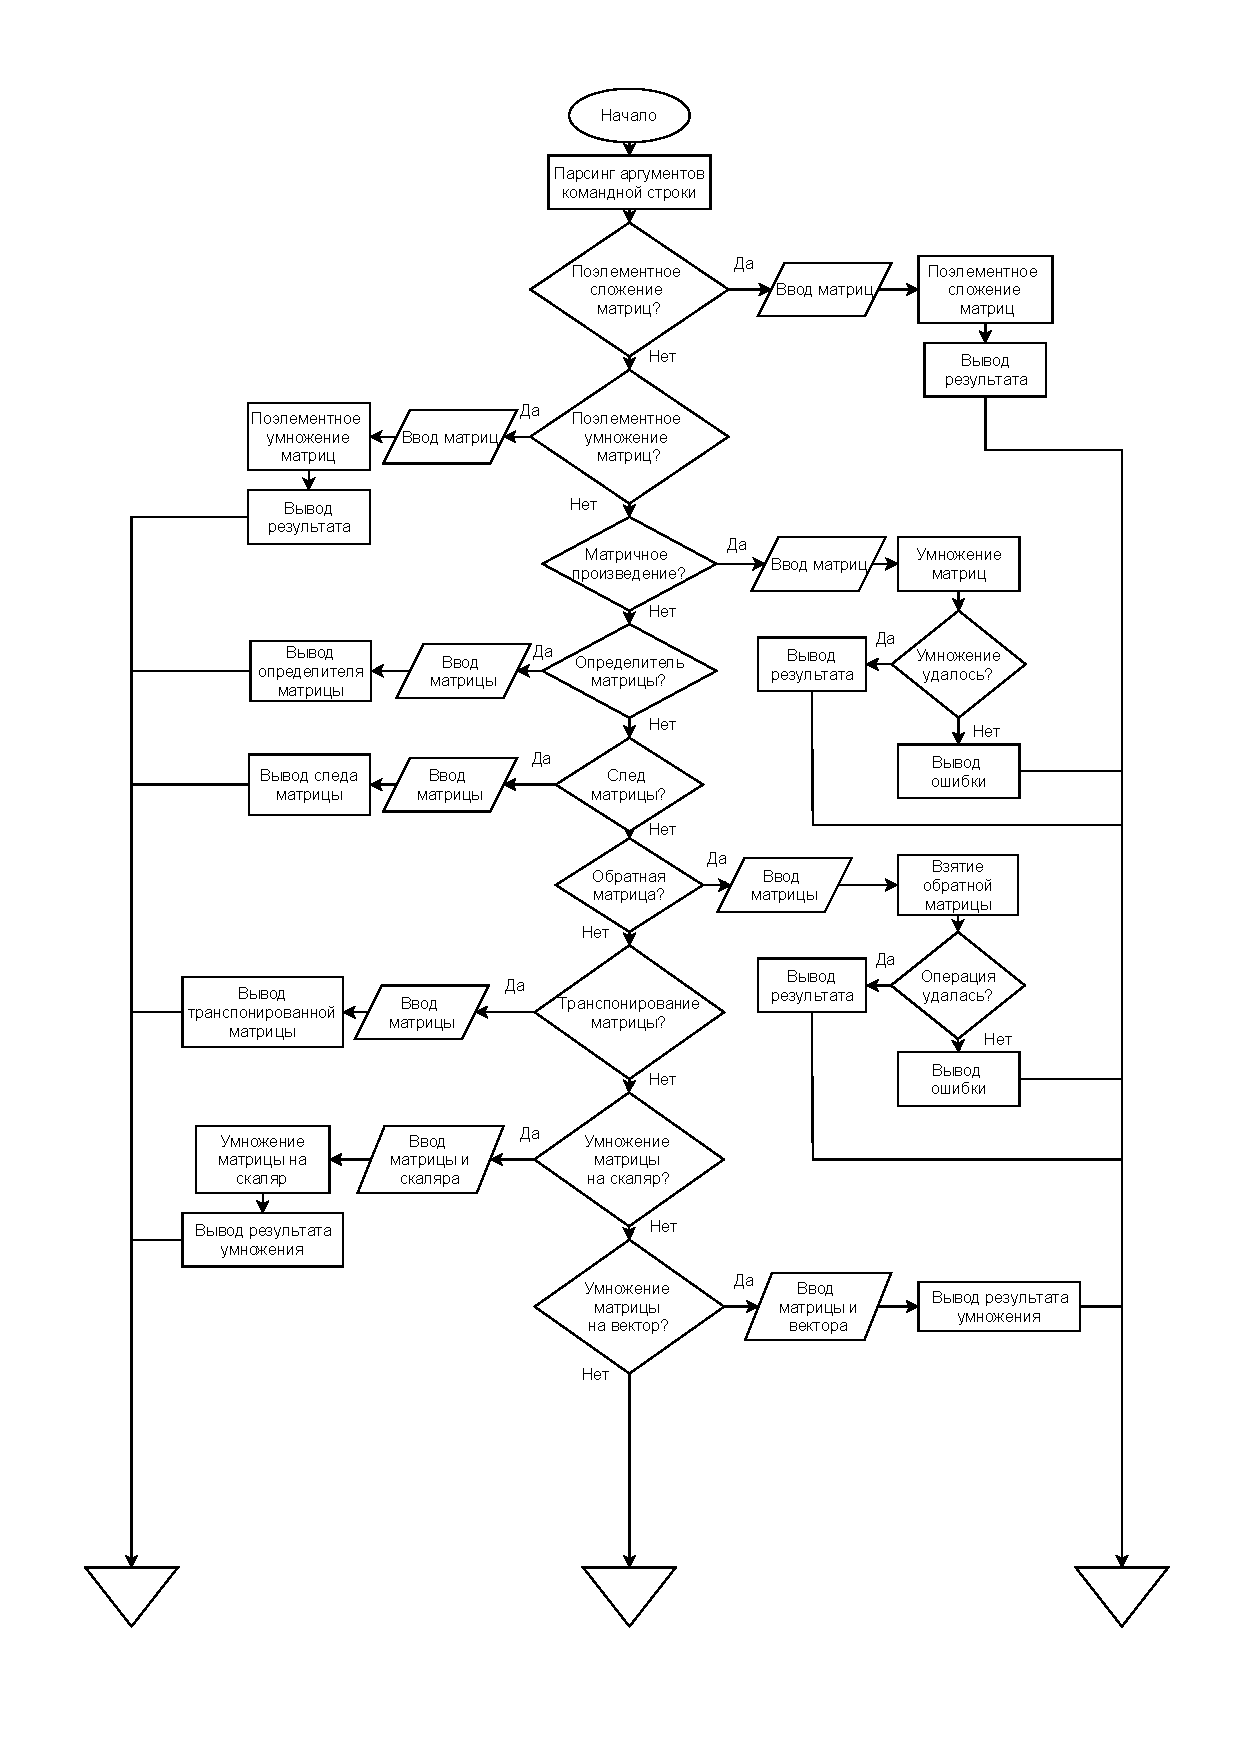
\includegraphics[page=1, width=\textwidth]{include/block_scheme.pdf}
	\caption{Блок-схема программы}
\end{figure}

\begin{figure}[H]
	\includegraphics[page=2, width=\textwidth]{include/block_scheme.pdf}
	\caption{Блок-схема программы}
\end{figure}

\begin{figure}[H]
	\includegraphics[page=3, width=\textwidth]{include/block_scheme.pdf}
	\caption{Блок-схема программы}
\end{figure}

\newpage

\section{Проверка работы программы}
Для проверки работоспособности программы испытаем 
несколько режимов работы для различных величин.

\vspace{0.1cm}

Взятие корня 4 степени из скаляра:
\begin{minted}[mathescape,linenos,breaklines]{bash}
./main.py scalar --sqrt 16 4
2.0
\end{minted}
 
Синус скаляра: 
\begin{minted}[mathescape,linenos,breaklines]{bash}
./main.py scalar --sin 1
0.8414709848078965
\end{minted}

Векторное произведение трехмерных векторов:
\begin{minted}[mathescape,linenos,breaklines]{bash}
./main.py vector -vm 
Введите первый вектор, элементы вводятся через запятую:
1,2,3
Введите второй вектор, элементы вводятся через запятую:
4,5,6
[-3.  6. -3.]
\end{minted}

Умножение вектора на скаляр:
\begin{minted}[mathescape,linenos,breaklines]{bash}
./main.py vector --mul_scal
Введите скаляр:
5 
Введите первый вектор, элементы вводятся через запятую:
1,2,3,4
\end{minted}

Транспонирование матрицы:
\begin{minted}[mathescape,linenos,breaklines]{bash}
./main.py matrix -t 
Введите матрицу, столбцы разделяются через ;, элементы - ,:
1,2,3;4,5,6
[[1. 4.]
 [2. 5.]
 [3. 6.]]
\end{minted}

Матричное произведение:
\begin{minted}[mathescape,linenos,breaklines]{bash}
./main.py matrix -mp 
Введите матрицу, столбцы разделяются через ;, элементы - ,:
1,2,3;4,5,6
Введите матрицу, столбцы разделяются через ;, элементы - ,:
1,2;3,4;5,6
[[22. 28.]
 [49. 64.]]
\end{minted}

\addcontentsline{toc}{section}{Выводы по работе}
\section*{Выводы по работе}
В ходе выполнения лабораторной работы была изучена библиотека NumPy для произведения различных математических операций, были получены навыки реализации ПО в объектно-ориентированном подходе.

\newpage

\addcontentsline{toc}{section}{Приложение}
\section*{Приложение}

\subsection*{UML-диаграмма}
\addcontentsline{toc}{subsubsection}{UML-диаграмма}
\begin{figure}[H]
	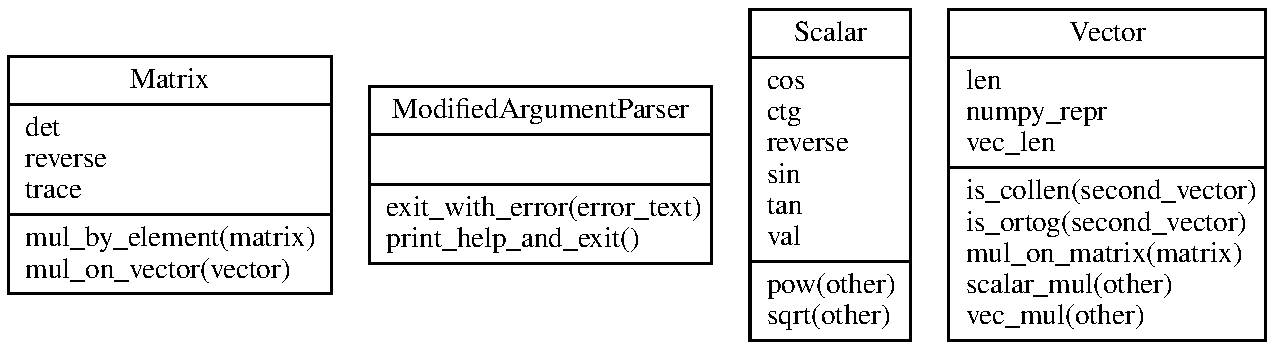
\includegraphics[width=\textwidth]{include/uml_diagram.pdf}
	\caption{UML-диаграмма программы}
\end{figure}

\subsection*{Листинг main.py}
\addcontentsline{toc}{subsubsection}{Листинг main.py}
\inputminted[mathescape,linenos,breaklines]{python}{../src/main.py}

\subsection*{Листинг math.py}
\addcontentsline{toc}{subsubsection}{Листинг math.py}
\inputminted[mathescape,linenos,breaklines]{python}{../src/models/math.py}

\subsection*{Листинг argparser.py}
\addcontentsline{toc}{subsubsection}{Листинг argparser.py}
\inputminted[mathescape,linenos,breaklines]{python}{../src/utils/argparser.py}

\subsection*{Листинг input.py}
\addcontentsline{toc}{subsubsection}{Листинг input.py}
\inputminted[mathescape,linenos,breaklines]{python}{../src/utils/input.py}

\end{document}          
